\documentclass[11pt,compress,t,notes=noshow, xcolor=table]{beamer}
\usepackage[]{graphicx}\usepackage[]{color}
% maxwidth is the original width if it is less than linewidth
% otherwise use linewidth (to make sure the graphics do not exceed the margin)
\makeatletter
\def\maxwidth{ %
  \ifdim\Gin@nat@width>\linewidth
    \linewidth
  \else
    \Gin@nat@width
  \fi
}
\makeatother

\definecolor{fgcolor}{rgb}{0.345, 0.345, 0.345}
\newcommand{\hlnum}[1]{\textcolor[rgb]{0.686,0.059,0.569}{#1}}%
\newcommand{\hlstr}[1]{\textcolor[rgb]{0.192,0.494,0.8}{#1}}%
\newcommand{\hlcom}[1]{\textcolor[rgb]{0.678,0.584,0.686}{\textit{#1}}}%
\newcommand{\hlopt}[1]{\textcolor[rgb]{0,0,0}{#1}}%
\newcommand{\hlstd}[1]{\textcolor[rgb]{0.345,0.345,0.345}{#1}}%
\newcommand{\hlkwa}[1]{\textcolor[rgb]{0.161,0.373,0.58}{\textbf{#1}}}%
\newcommand{\hlkwb}[1]{\textcolor[rgb]{0.69,0.353,0.396}{#1}}%
\newcommand{\hlkwc}[1]{\textcolor[rgb]{0.333,0.667,0.333}{#1}}%
\newcommand{\hlkwd}[1]{\textcolor[rgb]{0.737,0.353,0.396}{\textbf{#1}}}%
\let\hlipl\hlkwb

\usepackage{framed}
\makeatletter
\newenvironment{kframe}{%
 \def\at@end@of@kframe{}%
 \ifinner\ifhmode%
  \def\at@end@of@kframe{\end{minipage}}%
  \begin{minipage}{\columnwidth}%
 \fi\fi%
 \def\FrameCommand##1{\hskip\@totalleftmargin \hskip-\fboxsep
 \colorbox{shadecolor}{##1}\hskip-\fboxsep
     % There is no \\@totalrightmargin, so:
     \hskip-\linewidth \hskip-\@totalleftmargin \hskip\columnwidth}%
 \MakeFramed {\advance\hsize-\width
   \@totalleftmargin\z@ \linewidth\hsize
   \@setminipage}}%
 {\par\unskip\endMakeFramed%
 \at@end@of@kframe}
\makeatother

\definecolor{shadecolor}{rgb}{.97, .97, .97}
\definecolor{messagecolor}{rgb}{0, 0, 0}
\definecolor{warningcolor}{rgb}{1, 0, 1}
\definecolor{errorcolor}{rgb}{1, 0, 0}
\newenvironment{knitrout}{}{} % an empty environment to be redefined in TeX

\usepackage{alltt}
\newcommand{\SweaveOpts}[1]{}  % do not interfere with LaTeX
\newcommand{\SweaveInput}[1]{} % because they are not real TeX commands
\newcommand{\Sexpr}[1]{}       % will only be parsed by R
\newcommand{\xmark}{\ding{55}}%


\usepackage[english]{babel}
\usepackage[utf8]{inputenc}

\usepackage{dsfont}
\usepackage{verbatim}
\usepackage{amsmath}
\usepackage{amsfonts}
\usepackage{amssymb}
\usepackage{bm}
\usepackage{csquotes}
\usepackage{multirow}
\usepackage{longtable}
\usepackage{booktabs}
\usepackage{enumerate}
\usepackage[absolute,overlay]{textpos}
\usepackage{psfrag}
\usepackage{algorithm}
\usepackage{algpseudocode}
\usepackage{eqnarray}
\usepackage{arydshln}
\usepackage{tabularx}
\usepackage{placeins}
\usepackage{tikz}
\usepackage{setspace}
\usepackage{colortbl}
\usepackage{mathtools}
\usepackage{wrapfig}
\usepackage{bm}
\usepackage{amsmath}
\usepackage{pifont}

\usetikzlibrary{shapes,arrows,automata,positioning,calc,chains,trees, shadows}
\tikzset{
  %Define standard arrow tip
  >=stealth',
  %Define style for boxes
  punkt/.style={
    rectangle,
    rounded corners,
    draw=black, very thick,
    text width=6.5em,
    minimum height=2em,
    text centered},
  % Define arrow style
  pil/.style={
    ->,
    thick,
    shorten <=2pt,
    shorten >=2pt,}
}

\usepackage{subfig}

% Defines macros and environments
\usepackage{../../style/lmu-lecture}


\let\code=\texttt
\let\proglang=\textsf

\setkeys{Gin}{width=0.9\textwidth}

\setbeamertemplate{frametitle}{\expandafter\uppercase\expandafter\insertframetitle}

\usepackage{bbm}
% basic latex stuff
\newcommand{\pkg}[1]{{\fontseries{b}\selectfont #1}} %fontstyle for R packages
\newcommand{\lz}{\vspace{0.5cm}} %vertical space
\newcommand{\dlz}{\vspace{1cm}} %double vertical space
\newcommand{\oneliner}[1] % Oneliner for important statements
{\begin{block}{}\begin{center}\begin{Large}#1\end{Large}\end{center}\end{block}}


%new environments
\newenvironment{vbframe}  %frame with breaks and verbatim
{
 \begin{frame}[containsverbatim,allowframebreaks]
}
{
\end{frame}
}

\newenvironment{vframe}  %frame with verbatim without breaks (to avoid numbering one slided frames)
{
 \begin{frame}[containsverbatim]
}
{
\end{frame}
}

\newenvironment{blocki}[1]   % itemize block
{
 \begin{block}{#1}\begin{itemize}
}
{
\end{itemize}\end{block}
}

\newenvironment{fragileframe}[2]{  %fragile frame with framebreaks
\begin{frame}[allowframebreaks, fragile, environment = fragileframe]
\frametitle{#1}
#2}
{\end{frame}}


\newcommand{\myframe}[2]{  %short for frame with framebreaks
\begin{frame}[allowframebreaks]
\frametitle{#1}
#2
\end{frame}}

\newcommand{\remark}[1]{
  \textbf{Remark:} #1
}


\newenvironment{deleteframe}
{
\begingroup
\usebackgroundtemplate{
\includegraphics[width=\paperwidth,height=\paperheight]{../style/color/red.png}}
 \begin{frame}
}
{
\end{frame}
\endgroup
}
\newenvironment{simplifyframe}
{
\begingroup
\usebackgroundtemplate{
\includegraphics[width=\paperwidth,height=\paperheight]{../style/color/yellow.png}}
 \begin{frame}
}
{
\end{frame}
\endgroup
}\newenvironment{draftframe}
{
\begingroup
\usebackgroundtemplate{
\includegraphics[width=\paperwidth,height=\paperheight]{../style/color/green.jpg}}
 \begin{frame}
}
{
\end{frame}
\endgroup
}
% https://tex.stackexchange.com/a/261480: textcolor that works in mathmode
\makeatletter
\renewcommand*{\@textcolor}[3]{%
  \protect\leavevmode
  \begingroup
    \color#1{#2}#3%
  \endgroup
}
\makeatother





\input{../../latex-math/basic-math.tex}
\input{../../latex-math/basic-ml.tex}


\newcommand{\titlefigure}{figure/lm_reg2}
\newcommand{\learninggoals}{
\item Know the three components of a learner: Hypothesis space, risk, optimization 
\item Understand that defining these separately is the basic design of a learner
\item Know a variety of choices for all three components}


\title{Introduction to Machine Learning}
% \author{Bernd Bischl, Christoph Molnar, Daniel Schalk, Fabian Scheipl}
\institute{\href{https://compstat-lmu.github.io/lecture_i2ml/}{compstat-lmu.github.io/lecture\_i2ml}}
\date{}

\begin{document}


\lecturechapter{ML-Basics: Components of Supervised Learning}
\lecture{Introduction to Machine Learning}

% ------------------------------------------------------------------------------

\begin{vbframe}{Components of Supervised Learning}

Summarizing what we have seen before, many supervised learning algorithms 
can be described in terms of three components:

\lz

\begin{center}

  \textbf{Learning = Hypothesis Space + Risk + Optimization}
  
\end{center}

\lz

\begin{itemize}

  \item \textbf{Hypothesis Space:} Defines (and restricts!) what kind of model 
  $f$ can be learned from the data.
  
  \item \textbf{Risk:} Quantifies how well a specific model performs on a given 
  data set. This allows us to rank candidate models in order to choose the best one.
  
  \item \textbf{Optimization:} Defines how to search for the best model in the 
  \textbf{hypothesis space}, i.e., the model with the smallest \textbf{risk}.
  
\end{itemize}

\end{vbframe}

% ------------------------------------------------------------------------------

\begin{vbframe}{Components of Supervised Learning}

This concept can be extended by the concept of \textbf{regularization}, where the model complexity is accounted for in the risk:

\lz

%\begin{center}

  \textbf{Learning = Hypothesis Space + \invisible{xxxxxxxxx} Risk \invisible{ixxxxxx}+ Optim }
  \textbf{Learning = Hypothesis Space + Loss (+ Regularization) + Optim}
  
%\end{center}

\lz

\begin{itemize}

  \item For now you can just think of the risk as sum of the losses.
  
  \item While this is a useful framework for most supervised ML problems, it does not cover all special cases, because some ML methods are not defined via risk minimization and for some models, it is not possible (or very hard) to explicitly define the hypothesis space.
  
\end{itemize}

\end{vbframe}

% ------------------------------------------------------------------------------

\begin{frame}[squeeze]{Variety of Learning Components}

% \vskip -.5em
The framework is a good orientation to not get lost here:

\vskip .5em

\begin{footnotesize}

$\textbf{Hypothesis Space}: \begin{cases} 

\text{Step functions} \\
\text{Linear functions}\\
\text{Sets of rules}\\
\text{Neural networks}\\
\text{Voronoi tesselations}\\
\text{...}
\end{cases}$

$\phantom{Hypothesis Space RISK } \textbf{Risk / Loss}: \begin{cases}
\text{Mean squared error}\\
\text{Misclassification rate}\\
\text{Negative log-likelihood}\\
\text{Information gain}\\
\text{...}
\end{cases}$

$\phantom{hypothesis space risk RISK RISK RISK} \textbf{Optimization}: \begin{cases}
\text{Analytical solution}\\
\text{Gradient descent}\\
\text{Combinatorial optimization}\\
\text{Genetic algorithms}\\
\text{...}
\end{cases}$

\end{footnotesize}
\end{frame}


% ------------------------------------------------------------------------------

\begin{vbframe}{Supervised Learning, Formalized}

A \textbf{learner} (or \textbf{inducer}) $\inducer$ is a \emph{program} or 
\emph{algorithm} which

\begin{itemize}

  \item receives a \textbf{training set} $\D \in \allDatasets$, and,
  
  \item for a given \textbf{hypothesis space} $\Hspace$ of \textbf{models} 
  $f:\Xspace \rightarrow \R^g,$ 
  
  \item uses a \textbf{risk} function $\riskef$ to evaluate $f \in \Hspace$ on $\D$;\\ 
  or we use $\risket$ to evaluate f's parametrization $\thetab$ on $\D$
  
  \item uses an \textbf{optimization} procedure to find
      $$\fh = \argmin_{f \in \Hspace} \riskef \qquad \text{ or } \qquad \thetabh = \argmin_{\thetab \in \Theta} \risket.$$

\end{itemize}
So the inducer mapping (including hyperparameters $\bm{\lambda} \in \bm{\Lambda}$) is:
\[\inducer: \preimageInducerShort\rightarrow \Hspace\]
We can also adapt this concept to finding $\thetabh$ for parametric
models:
\[\inducer: \preimageInducerShort \rightarrow \Theta\]


%\lz 


%\lz

% {\footnotesize (This does not cover all special cases, but it's a useful framework for most supervised ML problems.)}

\end{vbframe}



% ------------------------------------------------------------------------------

\begin{vbframe}{Example: Linear Regression on 1D}

%So what could a learner look like? 
% Let us consider a regression task with 
% a single feature 

\begin{itemize}
  
  \item The \textbf{hypothesis space} in univariate linear regression is the set 
  of all linear functions, with $\thetab = (\theta_0, \theta_1)^\top$:
  
  $$\Hspace = \{\fx = \theta_0 + \theta \xv: \theta_0, \theta_1 \in \R \}$$
  
  \begin{center}
    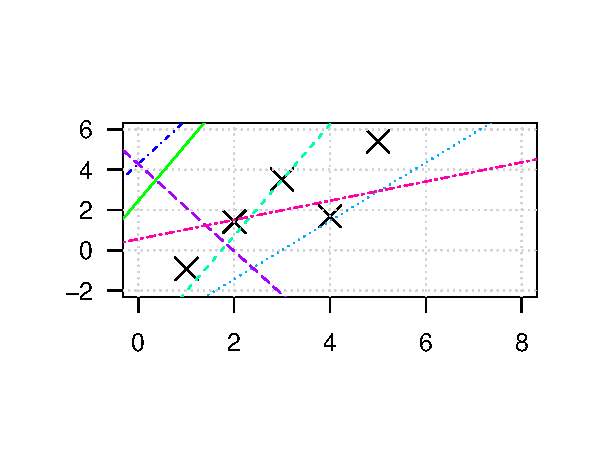
\includegraphics[trim = 1.5cm 1.5cm 1.5cm 1.5cm, width = 0.4\textwidth]{figure/lm_reg3} 
  \end{center}
\end{itemize}
  \textbf{Design choice:} We could add more flexibility by allowing polynomial effects or by using a spline basis.
  
  \framebreak
\begin{itemize}  
  \item We might use the squared error as loss function to our
  \textbf{risk}, punishing larger distances %between observations and regression line 
  more severely:
  
  $$\risket = \sumin (\yi - \theta_0 - \theta_1 \xi)^2$$
  
  \begin{center}
    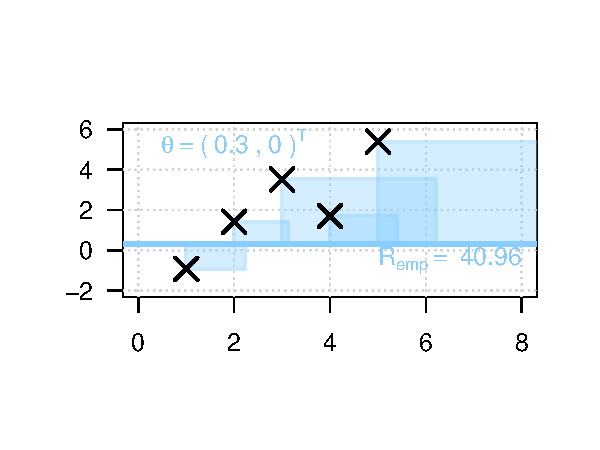
\includegraphics[trim = 1.5cm 1.5cm 1.5cm 1.5cm, width = 0.5\textwidth]{figure/lm_reg1} 
  \end{center}
\end{itemize}
  \textbf{Design choice:} Use absolute error / the $L1$ loss to create a more robust model which is less sensitive regarding outliers.
  
  \framebreak
\begin{itemize}  
  \item \textbf{Optimization} will usually mean deriving the 
  ordinary-least-squares (OLS) estimator $\thetabh$ analytically. 
  
    
\end{itemize}
\begin{figure}[!htb]
\minipage{0.49\textwidth}
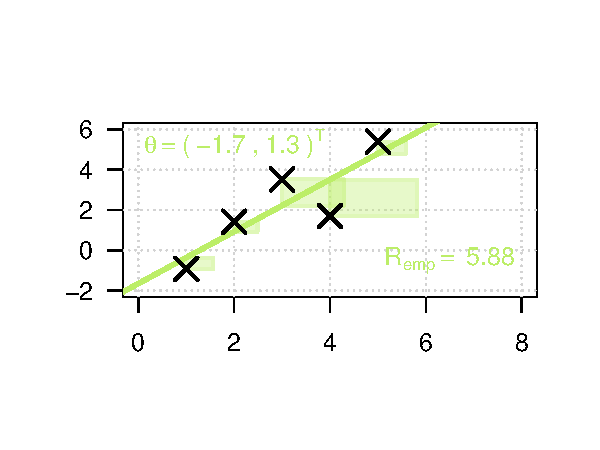
\includegraphics[trim=1.5cm 1.5cm 1.5cm 1.5cm, width=\linewidth]{figure/lm_reg2}  
\endminipage\hfill
\minipage{0.49\textwidth}
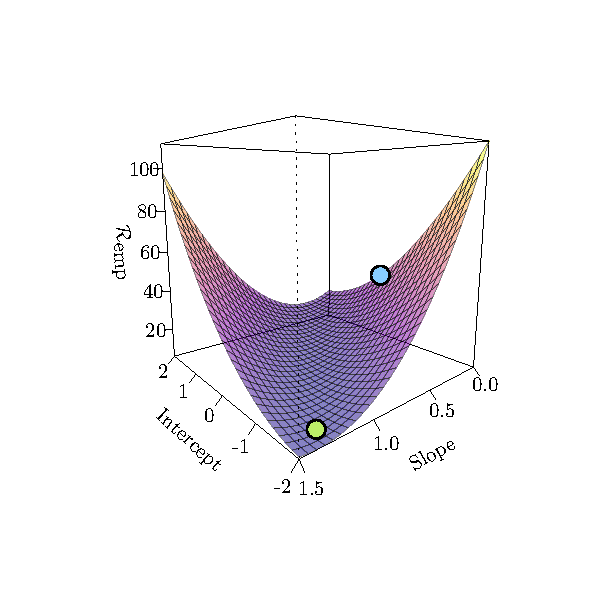
\includegraphics[trim=1.5cm 1.5cm 1.5cm 1.5cm, width=\linewidth]{figure/lm_reg4}
\endminipage
 
\end{figure}
  \textbf{Design choice:} We could use stochastic gradient descent to scale better to very large or out-of-memory data.

\end{vbframe}


% ------------------------------------------------------------------------------

\begin{vbframe}{Summary}

% \begin{itemize}

  By decomposing learners into these building blocks:

  \lz
  
  \begin{itemize}

    \item we have a framework to better understand how they work,
    
    \item we can more easily evaluate in which settings they may be more or less 
    suitable, and
    
    \item we can tailor learners to specific problems by clever choice of each 
    of the three components.
    
  \end{itemize}
  
  % \item There will, for instance, be optimization procedures that work well for
  % a certain combination of hypothesis space and risk function but perform poorly 
  % on others.
  
  % \item In fact, it is a commonly acknowledged problem that no universally best
  % learner exists.

% \end{itemize}

\lz

Getting this right takes a considerable amount of experience.

\end{vbframe}


% ------------------------------------------------------------------------------

\endlecture
\end{document}
